\chapter{ПЕРЕДАЧА ВИДЕОДАННЫХ В БЕСПРОВОДНЫХ ЦЕНТРАЛИЗОВАННЫХ СЕТЯХ}
\label{chap2}

\section{Вводные замечания}
\label{chap2:Intro}

Оптимизация передачи видеоданных наиболее актуальна для беспроводных систем связи по причине наличия ограничений на пропускную способность радиоканала, который считается <<узким местом>> (адаптированный перевод англоязычного термина <<bottle neck>>) сети в целом. Как следствие, скорость передачи информации от видео контент сервера до пользовательского устройства определяется именно скоростью передачи данных по радиоканалу. Основная проблематика всех исследований в области передачи видеоданных состоит не в предложении методов управления для телекоммуникационных сетей, а в обосновании их эффективности. Любое возможное управление может увеличить производительность системы, используя дополнительную информацию о передаваемом контенте, однако, в настоящее время не существует опорных теоретических исследований, с которыми возможно сравнить производительность предлагаемых решений.

В настоящее время наиболее распространены централизованные беспроводные системы связи с коммутацией пакетов, так как подобные системы позволяют добиться больших скоростей передачи информации и меньших задержек в беспроводном канале связи. Наиболее ярким представителем данного класса систем является стандарт The Long-Term Evolution (LTE)~\cite{opac-b1130916}.

Настоящий раздел посвящен задаче передачи видеоданных в современных централизованных беспроводных сетях. В разделе рассматривается специфика построения современных мобильных сетей связи, и решается задача формирования аналитической модели для проведения исследований подобных систем при передаче видеоданных. Предлагаемая модель состоит нескольких вложенных моделей, описание который последовательно будет представлено в настоящем разделе. В заключении раздела предлагается основополагающий результат, описывающий взаимосвязь между характеристиками сети, влияющими на ее производительность.

Основные результаты данного раздела опубликованы в работах...

\section{Структура современных беспроводных централизованных сетей передачи информации}
\label{chap2:WirelessSystemStructure}

В настоящее наибольшее распространение получили централизованные мобильные сети с коммутацией пакетов, так как они обеспечивают наиболее высокие скорости и малую задержку при передаче информации~\cite{Cisco}. В централизованных беспроводных сетях вся территория обслуживания разделена на зоны, называемые сотами. В каждой соте установлено устройство, управляющее передачей информацией всех активных пользователей в зоне его ответственности, называемое Базовой станцией. Базовая станция является программно-аппаратным комплексом обеспечивающим обмен информацией между пользователем в радиосети и остальной сетью передачи информации.

Современные беспроводные централизованные системы связи состоят из трех основных компонентов (рисунок~\ref{fig:LteStructure}):
\begin{itemize}
  \item \textit{Фиксированная магистральная сеть передачи данных}. Сеть передачи информации, в которая обеспечивает соединение с удаленными устройствами (в системах передачи видеоданных таким устройством является Видео Контент Сервер). Она характеризуется высокой надежностью, большой скоростью передачи информации, низкими задержкой и джиттром.
  \item \textit{Опорная сеть оператора}. Система устройств, обеспечивающая взаимодействие пользовательского устройства с удаленными узлами в фиксированной магистральной сети. Данный участок сети обладает схожими характеристиками с магистральной сетью.
  \item \textit{Радиосеть}. Беспроводная сеть передачи информации, организующая обмен данными между пользовательскими устройствами и остальными компонентами сети. Характеризуется несравнимо меньшими скоростями передачи информации и пропускными способностями каналов, большими задержкой и джиттером. Важной отличительной особенностью радиосети является изменяемость характеристик беспроводного канала передачи информации во времени.
\end{itemize}

\begin{figure}[htbp]
\begin{center}
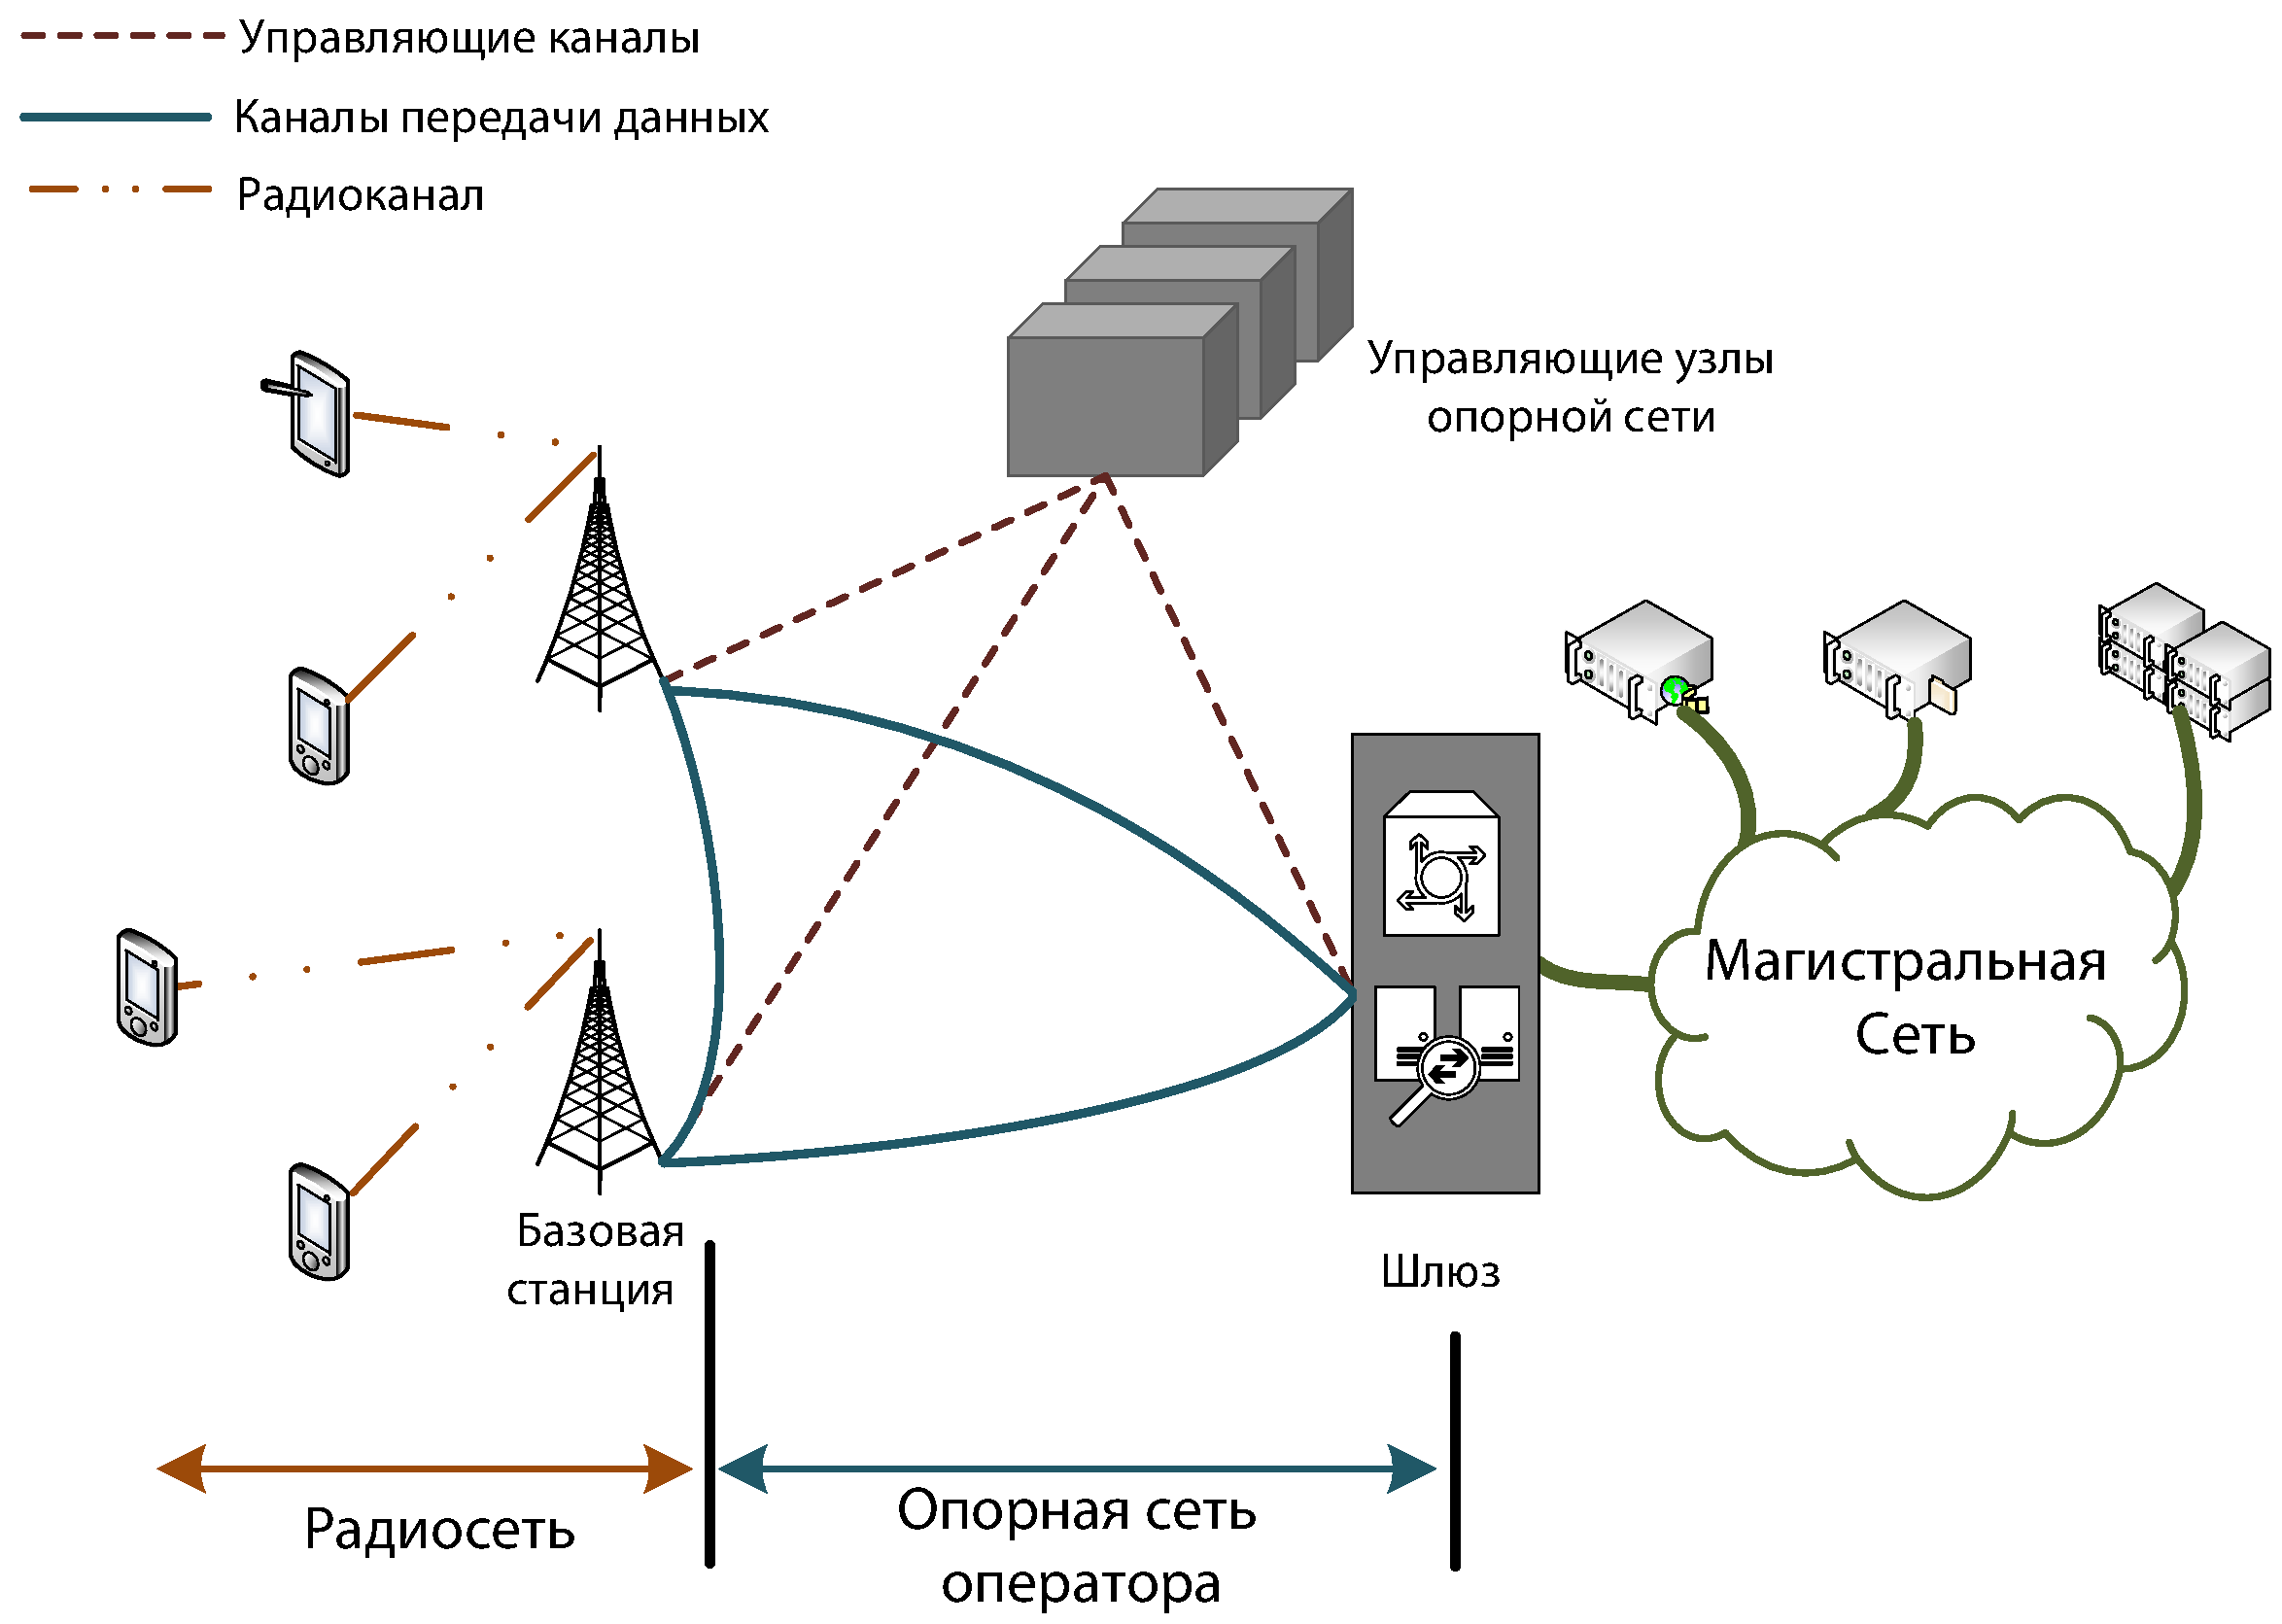
\includegraphics[width=\textwidth,height=0.4\textheight]{Chapter2/LteStucture.pdf}
\caption{Структура современных беспроводных централизованных систем}
\label{fig:LteStructure}
\end{center}
\end{figure}

Исходя из представленной выше структуры следует, что аналитическая модель должна агрегировать в себе множество аспектов и параметров, присущих беспроводным централизованным системам, что делает ее сложной и многоуровневой. Как следствие, дальнейшее представление будет разделено на несколько этапов, последовательно описывающих представленную структуру:
\begin{itemize}
  \item Общие положения предлагаемой модели;
  \item Модель радиосети:
  \begin{itemize}
  	\item Модель беспроводного канала передачи информации;
  	\item Модель базовой станции.
  \end{itemize}
  \item Модель воспроизводящего устройства.
\end{itemize}
В завершении описания будет представлена система используемых допущений.

\section{Общие положения аналитической модели}
\label{chap2:GeneralOverview}

В настоящей работе рассматривается система с конечным числом абонентов: в системе находятся $N$ пользователей, которые используют сервис просмотра видеоконтента. Каждый пользователь обладает устройством с установленным видеоплеером и характеризуется уникальным номером~--~$i$, однозначно ассоциируемым с воспроизводящим устройством (на рисунках обозначается сокращенно <<Устр.~$i$>>).

В современных централизованных беспроводных системах базовые станции в различных сотах работают независимо друг от друга: невозможна ситуация, когда одно и тоже устройство обслуживают несколько станций одновременно, так же решение о выделении ресурсов беспроводного канала принимается независимо, от работы базовых станций в соседних сотах. Следовательно, каждую соту возможно рассматривать как отдельную независимую систему, в которой необходимо производить оптимизацию передачи видео. На основании вышеизложенного, далее в работе будет рассматриваться работа только одной соты.

Все $N$ абонентов подключены по беспроводному каналу к одной базовой станции и имеют соединение с контент сервером, установленным в магистральной сети. Предполагается, что магистральные и опорные сети связи используют высокоскоростные каналы связи, что позволяет достигать колоссальных скоростей и минимально возможных задержек и джиттера при передаче информации. Таким образом, задержкой прохождение информации через данные участки сети можно пренебречь, и считать передачу данных через них мгновенной.

На удаленном видео контент сервере представлены видео различной длительности, каждое из которых представлено в некотором наборе битовых репрезентаций (подраздел~\ref{chap1:VideoFormat}). Каждое видео представлено в виде последовательности из сегментов равной длительности $d$ секунд. Длительность видеопоследовательностей на контент сервере является некоторой случайной величиной $m$. Репрезентация каждой видеопоследовательности однозначно сопоставляется с битовой скоростью потока. Далее в работе, для обозначения битовой скорости потока сегмента $j$, просматриваемого пользователем $i$, будет использоваться конструкция $R_{i,j}$. Предполагается, что все видеопоследовательности на контент сервере доступны в непрерывном отрезке битовых скоростей от $R_{min}$ до $R_{max}$:
\begin{equation}
R_{i,j} \in [R_{min}, R_{max}], i=\overline{1,N}.
\label{eq:BitrateConstr}
\end{equation}
В реальной системе непрерывность битовых скоростей может быть достигнута использованием на удаленном сервере траскодеров видеопотока. Траскодер~--~программный комплекс, позволяющий в режиме реального времени получать видеопоток с заданной битовой скоростью из потока с более высокой битовой скоростью. Использование траскодирования видеопотока позволяет видеоплееру подбирать битовую скорость видео под конкретные условия системы передачи видеоданных. Общая структура и особенности работы траскодеров видеопотока описаны в работах~\cite{1184336,1369700}.

Сегмент видеоданных $j$, при передаче через сеть пользователю $j$, представляется в виде последовательности из $P_{i,j}$ пакетов равного размера. Общий объем переданной информации сегмента $j$ на пользовательское устройство $i$ составляет $R_{i,j}\cdot d$ бит.

Введем модель, описывающую поведение пользователя при просмотре видеоконтента. Каждый абонент просматривает серию видео (рисунок~\ref{fig:UeBehaviorModel}) путем отправки запросов на видео контент сервер и последовательной загрузки сегментов видео данных через восходящий и нисходящий каналы связи соответственно. При заказе каждого сегмента видеоданных воспроизводящее устройство генерирует и отправляет на контент сервер уникальный запрос с указанием характеристик сегмента. В начале просмотра видео производится начальная буферизация, после окончания которой начинается демонстрация видеопотока и продолжится загрузка оставшихся видеоданных. После окончания просмотра видео пользователь $i$ через случайный интервал времени (паузу) $\tau_i$ закажет просмотр нового видео. Если скорости загрузки информации недостаточно для обеспечения просмотра видео, то могут возникнуть прерывания воспроизведения, вызванные необходимостью накопления достаточного объема видеоданных после опустошения буфера.

\begin{figure}[htbp]
\begin{center}
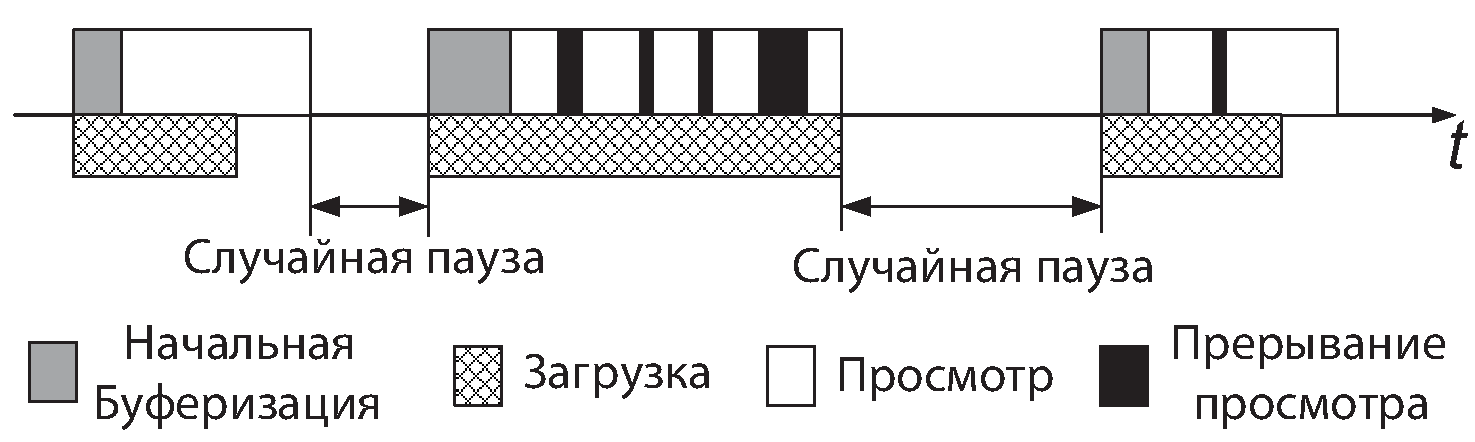
\includegraphics[width=\textwidth]{Chapter2/UeBehaviorModel.pdf}
\caption{Временная диаграмма поведения пользователя при просмотре видео}
\label{fig:UeBehaviorModel}
\end{center}
\end{figure}

Из модели поведения пользователя следует, что все время для конкретного пользователя можно разделить на три периода:
\begin{itemize}
	\item \textit{Буферизация}: пользователь ожидает начала или возобновления проигрывания видео (включает в себя начальные буферизации и прерывания воспроизведения, вызванные опустошением буфера);
	\item \textit{Просмотр}: штатное состояние, когда буфер на пользовательском устройстве достаточен и пользователь просматривает видеопоток;
	\item \textit{Пауза}: пользователь выбирает следующее видео для просмотра (в данном периоде просмотр и загрузка видео не осуществляются).
\end{itemize}
В дальнейшем будут использоваться конструкции $b_i^T$, $w_i^T$ и $p_i^T$ для обозначения общей длительности буферизации, просмотра и пауз пользователя $i$ за время в отрезке $[0, T]$ соответственно.

На уровне пользователя данную модель поведения возможно описать двумя основными характеристиками: коэффициентом разряженности видеопотока и отношением длительности буферизации к длительности просмотра для каждого конкретного пользователя.

\begin{definition}
\label{def:VideoSparseness}
    \emph{Коэффициент разряженности видеопотока пользователя $i$}~--~это отношение суммы длительностей просмотра и пауз к длительности просмотра пользователя $i$ за интервал времени $T\rightarrow\infty$:
    $$\gamma_i = \lim\limits_{T\rightarrow\infty} \frac{w_i^T + p_i^T}{w_i^T}.$$
\end{definition}

По определению коэффициент разряженности потока является величиной большей или равной единице: $\gamma_i \geq 1, i=\overline{1,N}$. Данное значение описывает активность пользователя при просмотре видео и показывает взаимосвязь между общим временем просмотра и пауз для конкретного абонента. Например, сравним двух пользователей $l$ и $r$, которые просмотрели одинаковую длительность видео за время $T$, однако $\gamma_l > \gamma_r$, это означает что пользователь $l$ делал большие паузы между просмотрами видео, чем пользователь $r$.

\begin{definition}
\label{def:BWTR}
    \emph{Отношение длительности буферизации к просмотру}~--~это отношение общей длительности буферизации к длительности просмотра пользователя $i$ за интервал времени $T\rightarrow\infty$:
    $$q_i = \lim\limits_{T\rightarrow\infty} \frac{b_i^T}{w_i^T}.$$
\end{definition}

По определению занчение отношения времени буферизации к просмотру для каждого пользователя является неотрицательной величиной: $q_i \geq 0, i=\overline{1,N}.$ Исходя из подраздела \ref{chap1:VideoMOS}, буферизация является негативным эффектом воспроизведения видео, который имеет критично большое влияние на качество восприятия абонентом сервиса передачи видеоданных. Как следствие, данный критерий обладает обратной корреляцией с удовлетворенности пользователя: чем больше значение $q_i$, тем меньше удовлетворенность пользователя.

\section{Модель беспроводного канала передачи информации}
\label{chap2:RadioChannel}

Одно из важнейших положений в описании представляемой аналитической модели занимает модель радиосети. В современных централизованных беспроводных системах радиосеть состоит из трех основных компонентов:
\begin{itemize}
	\item Беспроводной канал передачи информации;
	\item Базовая станция;
	\item Пользовательское устройство.
\end{itemize}

В начале будет описана структура и аспекты работы беспроводного канала передачи информации. В существующих беспроводных централизованных сетях на физическом уровне ресурсы задаются двумя измерениями: частотой и временем (рисунок~\ref{fig:LteRadioChannel}). Во временной области все время работы разделено на периоды равной длительности, называемые слотами. Типовая длительность одного слота равняется 1-й миллисекунде (мс). В англоязычной литературе для обозначения слота используется Slot или Transmission Time Interval (TTI), обозначающие минимальное дробление времени для передачи информации. В частотной области вся полоса передачи информации разделена на области равной ширины, в современных стандартах передачи информации ширина данных областей равняется 180 кГц. Минимальной единицей ресурсов является Ресурсный Блок~--~одна частотная область длительностью в один слот.

Множество ресурсных блоков формируют общий канал передачи информации, ресурсы которого могут быть распределены между пользователями в радиосети. Помимо общего канала связи реализованы служебные каналы, решающие задачи поддержания синхронизации и управление передачей пользовательских устройств, оценки качества канала, обеспечения надежной передачи информации по ненадежному каналу и т.д. Данные каналы занимают ресурсы в начале и внутри ресурсных блоков.

\begin{figure}[htbp]
\begin{center}
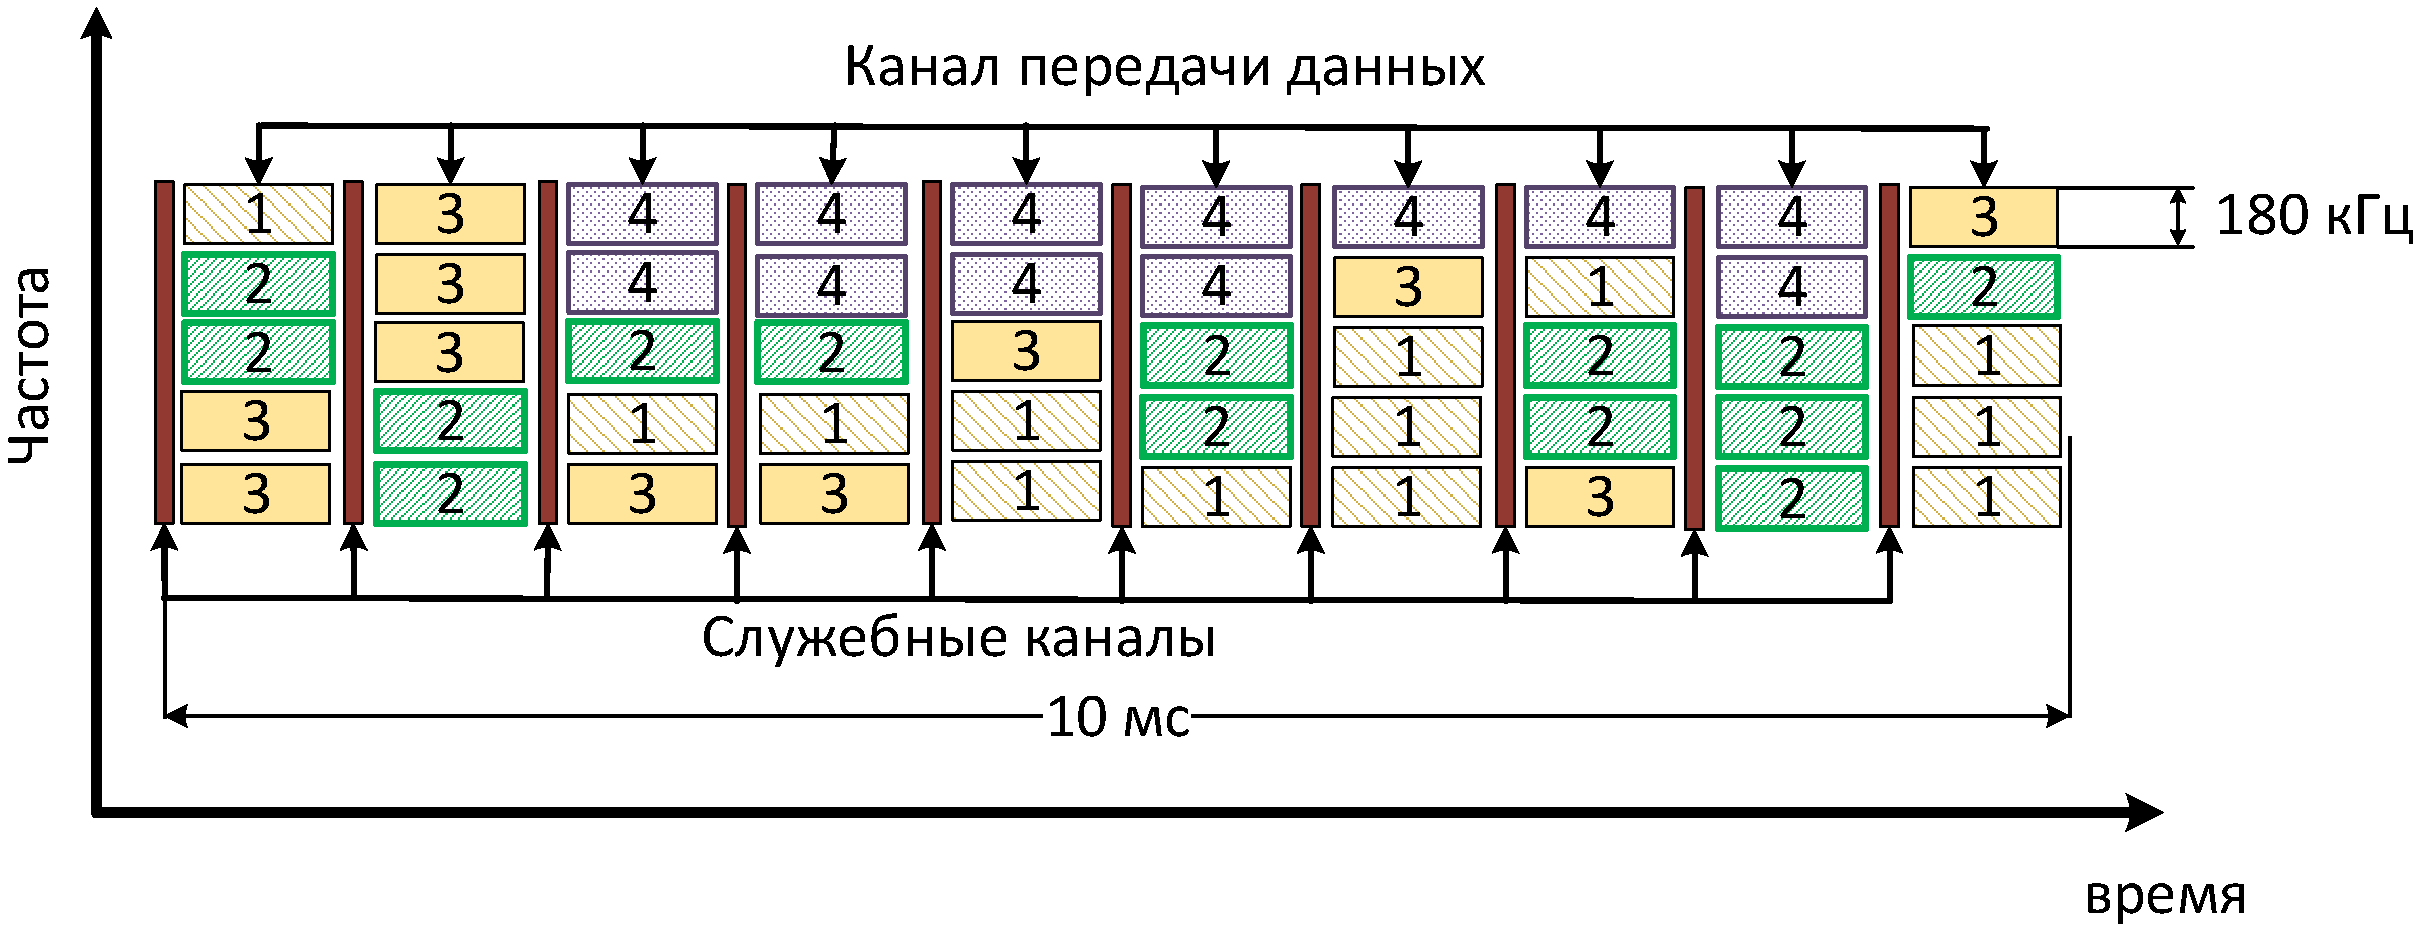
\includegraphics[width=\textwidth]{Chapter2/LteRadioChannel.pdf}
\caption{Структура беспроводного канала}
\label{fig:LteRadioChannel}
\end{center}
\end{figure}

Важной отличительной особенностью беспроводных каналов связи является изменчивость его характеристик как во времени, так и в частотной области. Подобная изменчивость вызвана наличием помех от работы других систем связи, движением пользователя и окружения, и т.д. Данный факт приводит к тому, что для одного абонента в разных ресурсных блоках может быть передан различный объем информации. Для каждого ресурсного блока на базовой станции вычисляется затухание распространения сигнала на основе информации от служебных каналов связи. Для описания качества канала на вышележащих уровнях базовой станции, полученное значение затухания сигнала для конкретного ресурсного блока и абонента преобразуется в кодо-модуляционную схему. Кодо-модуляционная схема (Modulation Code Scheme или MCS)~--~целое число в отрезке от 0 до 28, описывающее используемую модуляцию (QPSK, QAM-16, QAM-64) и настройки помехоустойчивого кодирования. Значение кодо-модуляционной схемы имеет прямую корреляцию с уровнем качества канала: чем выше значение MCS, тем выше качество канала. Используемая кодо-модуляционная схема определяет количество байт, которое возможно передать в конкретном ресурсном блоке.

Рассматриваемая модель предполагает, что пользователи в соте могут находится в различных условиях беспроводного канала, вызванные удаленностью от базовой станции. Последовательно рассмотрим восходящий и нисходящий беспроводные каналы. В современных централизованных системах связи восходящий канал обладает сравнимыми характеристиками с нисходящим, однако, его загруженность несравнимо меньше по сравнению с нисходящей линией связи. Как следствие, в предлагаемой модели восходящий радиоканал считается абсолютно надежным и задержкой передачи запросов на сегменты видео можно пренебречь.

Аналитическая модель уделяет большое внимание нисходящему каналу связи, так как от его производительности зависит удовлетворенность пользователей в соте. В данной работе рассматривается модель канала, обладающая следующим свойством: затухание при распространении сигнала происходит одинаково по всей ширине полосы передачи информации для конкретного пользователя в одном моменте времени. В реальной системе данное допущение приводит к равенству значений выбранных кодо-модуляционных схем для всех ресурсных блоков в рамках одного слота конкретного пользователя. Следствием равенства кодо-модуляционных является равенство возможного передаваемого объема информации для всех ресурсных блоков в слоте.

Таким образом, состояние беспроводного канала пользователя $i$ возможно охарактеризовать максимально достижимой скоростью канала.
\begin{definition}
\label{def:MaxThroughput}
    \emph{Максимально достижимая скорость канала пользователя $i$}~--~скорость передачи информации по беспроводному каналу, если все доступные ресурсы были выделены $i$-му пользователю.
\end{definition}
Данная величина является аналогичной скорости передачи данных, при условии, что пользователь $i$ находится один в соте. Далее в работе, для обозначения максимально достижимой скорости канала пользователя $i$ будет использоваться конструкция $C_i$, а для сокращения текста слово <<максимальная>> будет опускаться.

Обобщая сказанное ранее, для каждого пользователя $i$ существует случайный процесс изменения затухания распространения сигнала от времени $L_i(t)$. На основе значения $L_i(t)$ в момент времени $t$ на базовой станции подбирается кодо-модуляционная схема, таким образом, что вероятность ошибки при передаче информации является пренебрежимо малой. Выбранная кодо-модуляционная схема определяет максимальную пропускную канала $C_i(t)$ в момент времени $t$.

Предполагается, что состояние беспроводного канала изменяется, таким образом, что в течении загрузки пакета $k$ из сегмента $j$ максимально достижимая скорость канала пользователя $i$ постоянна:
\begin{equation}
\left.C_i(t)\right\vert^{t_{i,j,k}+\Delta t_{i,j,k}}_{t_{i,j,k}}=C_{i,j,k},
\label{eq:ChannelConst}
\end{equation}
где $t_{i,j,k}$~--~момент времени начала загрузки пользователем $i$ пакета $k$ из сегмента $j$, $\Delta t_{i,j,k}$~--~длительность загрузки пользователем $i$ пакета $k$ из сегмента $j$, $C_{i,j,k}$~--~максимально достижимая скорость канала пользователя $i$ в течении загрузки пакета $k$ из сегмента $j$.

Для современных централизованных беспроводных сетей в типовой соте для передачи информации в одном слоте доступны 48 ресурсных блоков (ширина полосы 10 МГц), и при использовании кодо-модуляционной схемы с модуляцией QPSK в одном слоте возможно передать 900 байт полезной информации. Таким образом, для пользователя в плохих радиоусловиях пакет может быть передан за 2 миллисекунды (подраздел~\ref{chap1:VideoFormat}). Данный факт демонстрирует, что представленное ограничение не сужает возможную сферу применения предлагаемой модели беспроводного канала.

Так же введем дополнительное обозначение $C_{i,j}^{-1}$ равное выборочному среднему для величин обратных к максимально достижимой скорости при передачи пакетов в течение одного сегмента видеоданных:
\begin{equation}
\nonumber
C_{i,j}^{-1} = \frac{1}{P_{i,j}}\sum\limits_{k=1}^{P_{i,j}} \frac{1}{C_{i,j,k}},
\label{eq:ChannelConst_v1}
\end{equation}
где $P_{i,j}$~--~число пакетов в сегменте $j$ пользователя $i$.

\section{Распределение ресурсов беспроводного канала связи}
\label{chap2:Scheduler}

После определения структуры беспроводного канала необходимо привести описание того как, используя данную структуру, происходит обмен данными между базовой станций и пользовательским устройством. Для этого рассмотрим функциональную структуру базовой станции.

Основной задачей базовой станции, является организация надежной передачи информации по ненадежному радиоканалу. Для решения данной задачи используется структура, состоящая из четырех уровней (рисунок~\ref{fig:eNbLayers}):
\begin{itemize}
	\item Уровень обработки пакетов;
	\item Уровень очередей для передачи информации по беспроводному каналу связи;
	\item Уровень доступа ко среде передачи информации;
	\item Уровень физической среды.
\end{itemize}

\begin{figure}[htbp]
\begin{center}
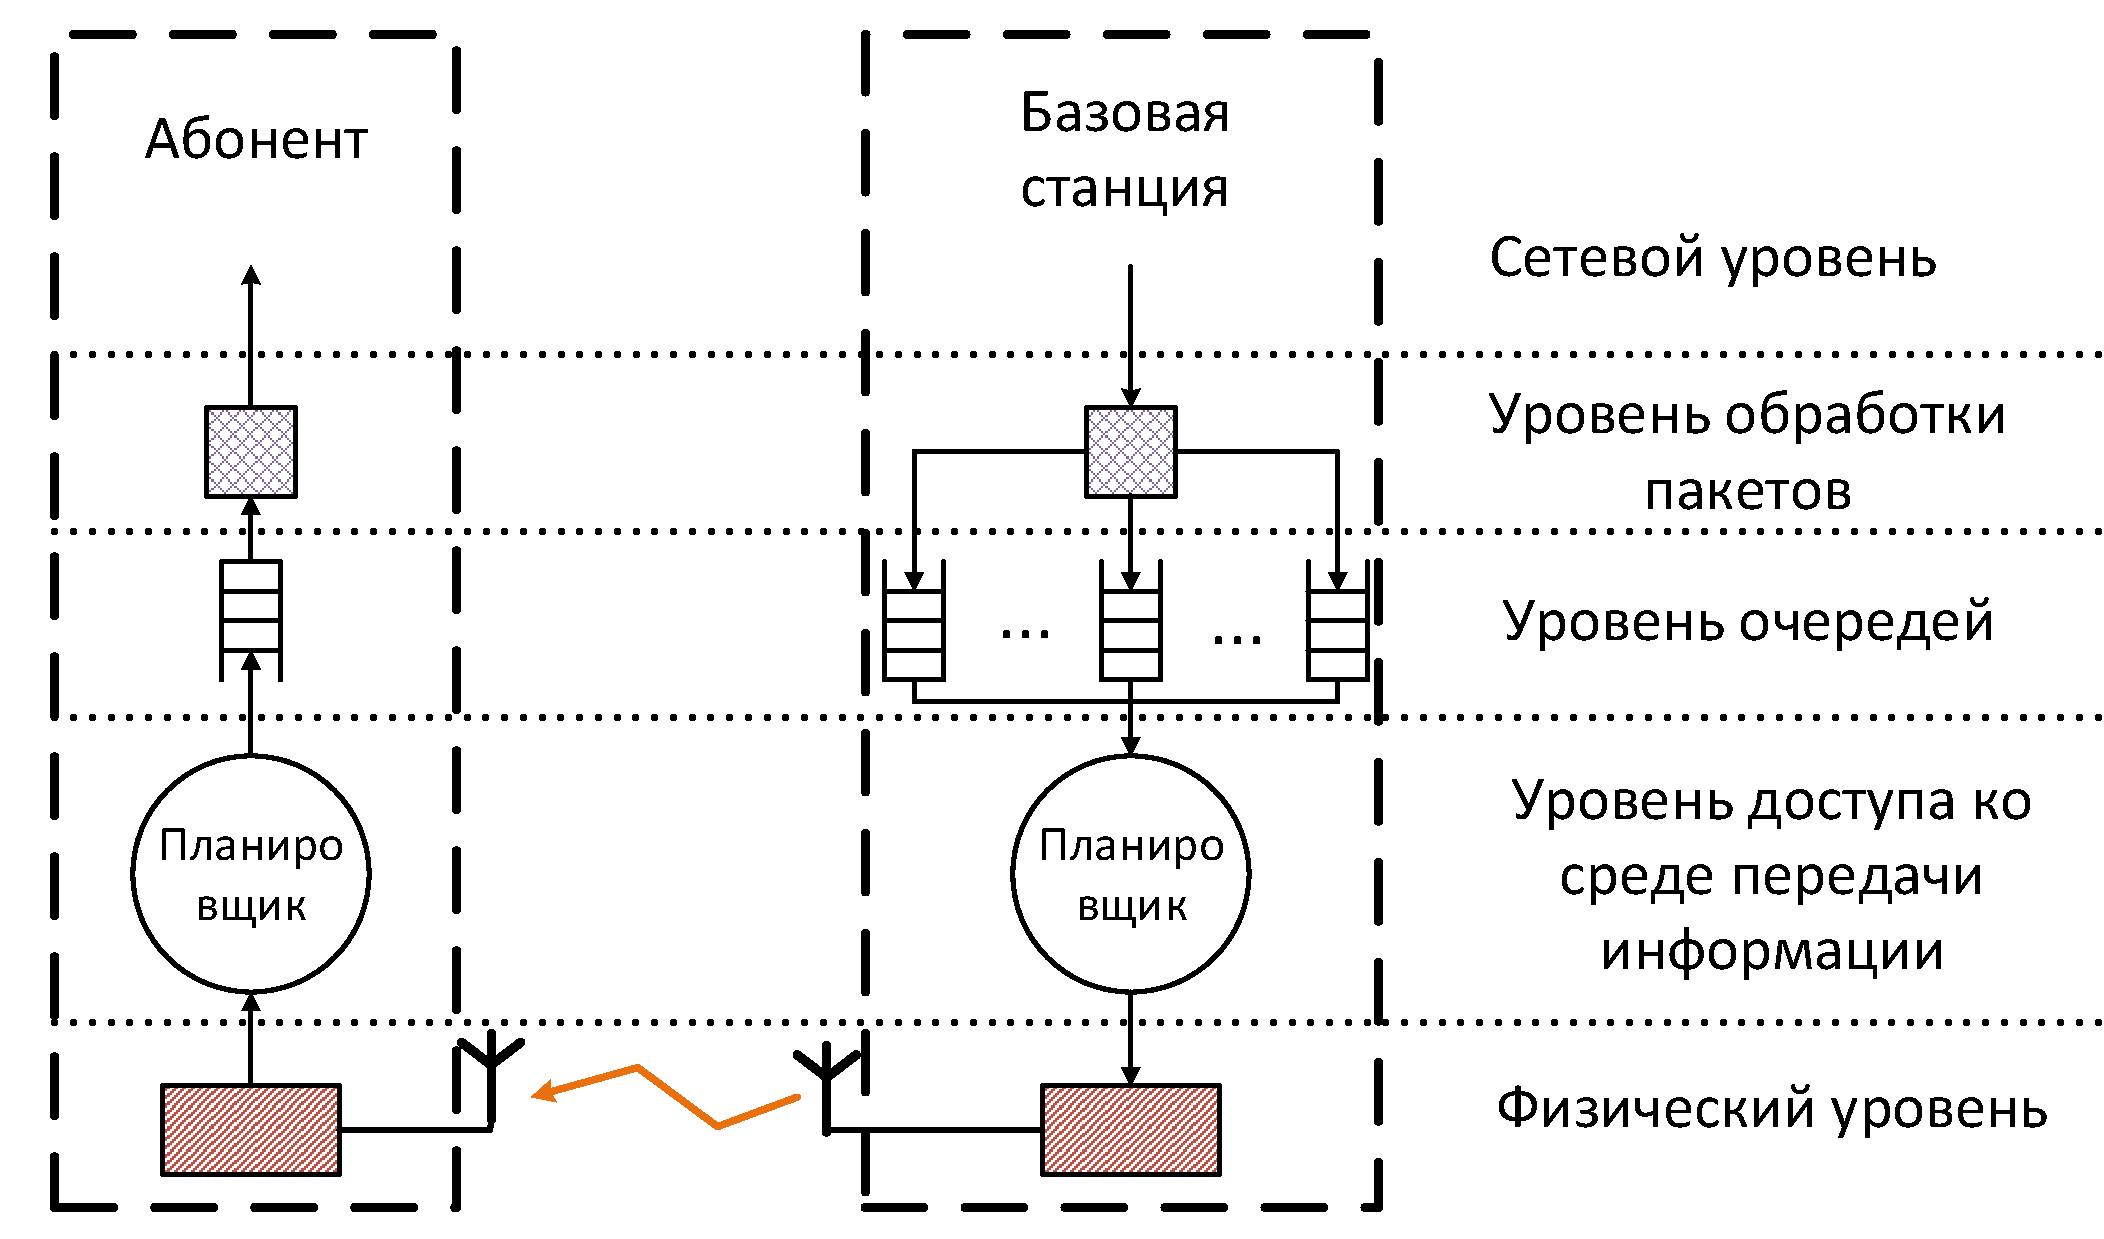
\includegraphics[width=\textwidth,height=0.4\textheight]{Chapter2/eNbLayers.pdf}
\caption{Функциональная структура базовой станции и пользовательского устройства}
\label{fig:eNbLayers}
\end{center}
\end{figure}

Произведем описание доставки пакета с данными от момента его получения на базовой станции, до момента его появления на сетевом уровне пользовательского устройства. Из опорной сети оператора пакет попадает на уровень обработки пакетов, данный уровень выполняет две функции. Первой функцией является сжатие заголовков пакетов транспортного и сетевого уровня, для уменьшения объема передаваемой информации по беспроводному канала. Реализация сжатия заголовков пакета позволяет нивелировать накладные издержки при передачи информации по беспроводному каналу и считать, что в пакете нет никакой избыточности, добавляемой сетевыми протоколами. Второй функцией является определение абонента и передача информационной части пакета в его очередь на нижележащем уровне.

Ниже расположен уровень очередей для передачи информации по беспроводному каналу связи. На данном уровне для каждого пользователя, подключенного к базовой станции, расположена очередь (буфер) для информации. Уровень очередей является промежуточным между уровнями обработки пакетов и доступа к среде передачи информации, выполняющего роль временного хранилища информации при ее передачи по беспроводному каналу. Обслуживанием очередей занимается нижележащий уровень: уровень доступа ко среде передачи (Medium Access Control или MAC).

Уровень доступа ко среде передачи информации решает ключевую задачу для системы в целом: на основе информации от уровня физической среды и вышележащих уровней базовой станции произвести распределение ресурсов беспроводного канала и обеспечить надежность передачи информации. Решением данной задачи занимается планировщик ресурсов беспроводного канала, установленный на базовой станции (в англоязычной литературе используется обозначение Media Access Channel Scheduler или MAC Scheduler). Далее в работе для сокращения объема текста в качестве обозначения <<планировщика ресурсов беспроводного канала>> будет использоваться термин <<планировщик>>.

Планировщик в каждом слоте производит распределение ресурсов радиоканала (ресурсных блоков) в соответствие с некоторым алгоритмом. Важно отметить, что планировщик не выделяет ресурсы абонентам, у которых нет данных в данном слоте. В каждом слоте формируется карта распределения ресурсных блоков, которая будет передана на физический уровень. На рисунке~\ref{fig:LteRadioChannel} представлен пример распределения ресурсов в течении десяти слотов для четырех активных пользователей. Таким образом, работу алгоритма планирования можно представить в виде распределения долей канала между пользователями. Например, в первом слоте пользователям $1$, $2$ и $3$ были выделены доли беспроводного канала $0.2$, $0.4$ и $0.4$ соответственно.

Сформированная карта распределение ресурсных блоков будет передана на уровень физической среды, который обеспечит передачу информации из уровня очередей в выделенных частотно-временных ресурсах. В дальнейшем, при корректной работе всех описанных уровней базовой станции пакет будет доставлен по беспроводному каналу на пользовательское устройство и, пройдя стек уровней в обратном порядке, станет доступен на сетевом уровне пользовательского устройства.

Несмотря на важную роль планировщика, алгоритмы планирования не стандартизованы для существующих систем связи, поэтому каждый производитель базовых станций использует собственные реализации алгоритмов планирования. Создание подобных алгоритмов алгоритмов является открытой задачей, так как требования к ним очень обширны и не существует строгих теоретических исследований о их максимальной производительности. В настоящее время известны два эвристических алгоритма планирования ресурсов: Proportional Fair и Round Robin. Алгоритм планирования Proportional Fair ставит своей задачей обеспечения равных скоростей передачи информации для всех активных пользователей. Алгоритм планирования Round Robin обеспечивает равный доступ к ресурсам радиоканала для всех активных пользователей. Поэтому настоящая диссертационная работа ставит своей основной задачей исследование алгоритмов планирования, с целью увеличения их производительности и, как следствие, всей беспроводной централизованной сети для передачи видеоданных.

Центральное положение, в представляемой аналитической модели, занимает алгоритм планирования распределения ресурсов беспроводного канала, установленный на базовой станции. Введем определение алгоритма планирования:

\begin{definition}
\label{def:SchedulingAlg}
    \emph{Алгоритм планирования}~--~это правило, в соответствии с которым базовая станция в момент времени $t$ распределяет доли ресурсов беспроводного канала $\alpha_i(t)$ для пользователя $i$.
\end{definition}

Таким образом, работу алгоритма планирования в момент времени $t$ возможно описать набором функций: ${A}(t) = \left\{\alpha_{i}(t), i = \overline{1,N}\right\}$. Очевидным ограничением на возможные значения функций $\alpha_i(t)$ является следующее неравенство:
\begin{equation}
\forall t: \sum\limits_{i=1}^{N}\alpha_{i}(t) \leq 1.
\label{eq:sumAlpha}
\end{equation}
Неравенство (\ref{eq:sumAlpha}) может быть интерпретировано следующим образом: в любой момент времени работы алгоритма планирования общий объем выделенных ресурсов не превышает доступного объема ресурсов для канала передачи информации. Следовательно, для любого пользователя $i$, мгновенная скорость передачи информации в нисходящем канале связи $S_i(t)$ может быть вычислена следующим образом:
\begin{equation}
S_i(t) = \alpha_i(t) C_i(t).
\label{eq:MomentRate}
\end{equation}

Алгоритм планирования в каждый момент времени решает задачу распределения ресурсов беспроводного канала. Для решения данной задачи ему доступна информация о предыстории, а именно доли выделенных ресурсов канала, значения максимально достижимых скоростей канала и объем переданной информации для каждого пользователя:
\begin{equation}
\overline{A}(t) = \mathcal{A}\left( S_i(\tau), C_i(\tau);\tau<t, i=\overline{1,N} \right),
\label{eq:SchedulingRule}
\end{equation}
где $\mathcal{A}\left(\cdot\right)$ является алгоритмом планирования. В формуле (\ref{eq:SchedulingRule}) информация о предыстории выделенных долей беспроводного канала и объемах переданной информации для пользователя $i$ агрегированы в значении $S_i(\tau)$, так как данные параметры задаются соотношением (\ref{eq:MomentRate}).

Важно отметить факт, что для планировщика базовой станции пользователь в каждый момент времени может находиться в одном из двух состояний: активном и неактивном. Пользователь считается активным, если у данного пользователя есть информация для передачи в нисходящем канале на базовой станции, иначе пользователь считается неактивным. В реальной системе, активность абонента так же определяется на основе заполненности очередей. Основываясь на модели поведения пользователя при просмотре видео, пользователь может является активным только в период осуществления загрузки данных (рисунок~\ref{fig:UeBehaviorModel}). Важно отметить, что загрузка информации состоит из последовательной передачи пакетов с видеоданными, и пользователь считается неактивным во время пауз между их загрузками.

В данной диссертационной работе рассматриваются алгоритмы планирования, которые удовлетворяют представленному ниже набору свойств:
\begin{itemize}
	\item В каждый момент времени активному пользователю гарантировано выделение минимальной доли ресурсов канала $\alpha_{i}^{min}$:
	\begin{equation}
		\label{eq:MinGuarPart}
		\begin{cases}
			\alpha_i(t) = 0, & \text{пользователь $i$ неактивен в момент времени $t$} \\
			\alpha_i(t) \geq \alpha_{i}^{min}, & \text{пользователь $i$ активен в момент времени $t$}\\
		\end{cases}.
	\end{equation}
	Минимальная доля ресурсов канала является величиной, отличной от нуля: $\alpha_{i}^{min} > 0$, и сумма минимальных долей ресурсов канала для всех пользователей не превышает общего объема ресурсов, доступных для планирования: $\sum\limits_{i=1}^{N}\alpha_{i}^{min} \leq 1$.
	\item Ресурсы беспроводного канала не могут быть выделены неактивному абоненту.
	\item В каждый момент времени планировщик распределяет все доступные ресурсы между активными абонентами:
\end{itemize}
\begin{equation}
	\label{eq:AllResources}
	\sum\limits_{i=1}^{N}\alpha_{i}(t) =
	\begin{cases}
		0, & \text{в момент времени $t$ все пользователи неактивны} \\
		1, & \text{иначе}\\
	\end{cases}.
\end{equation}

\section{Модель воспроизводящего устройства}
\label{chap2:VideoTrafficModel}

В завершении представлении аналитической модели будет определена модель видеотрафика и видиоплеера. В данной работе предполагается, что видеоплеер и видео контент сервер поддерживают технологию адаптивной передачи видеоконтента DASH (подраздел~\ref{chap1:VideoPlayers}) (рисунок~\ref{fig:PlayerModel}). Видеоплеер, установленный на пользовательском устройстве, осуществляет последовательную загрузку сегментов видеопоследовательности: следующий сегмент видео может быть заказан после окончания загрузки предыдущего и некоторой задержки. Пауза между заказами обусловлены стратегией наполнения буфера и моделью поведения пользователя. Данная задержка может быть короткой, если загружается сегмент в середине видео и достаточной длинной, если загружается первый сегмент, в случае если данная задержка включает в себя случайную паузы между просмотрами видеопоследовательностей, представленные на рисунке~\ref{fig:UeBehaviorModel}.

\begin{figure}[htbp]
\begin{center}
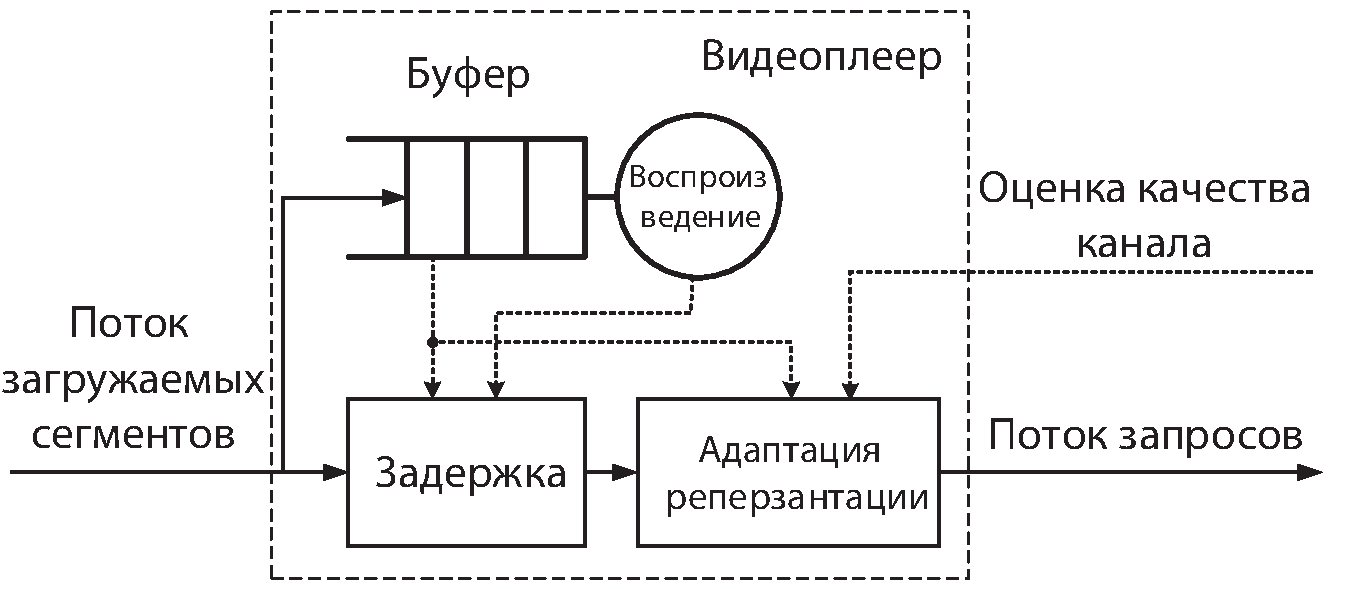
\includegraphics[width=0.8\textwidth]{Chapter2/PlayerModel.pdf}
\caption{Модель воспроизводящего устройства}
\label{fig:PlayerModel}
\end{center}
\end{figure}

При заказе нового сегмента видеопоследовательности видеоплеер решает задачу выбора репрезентации для заказываемого сегмента. В предлагаемой модели репрезентация сегмента однозначно сопоставлена с битовой скоростью, таким образом задача выбора репрезентации сводится к задаче адаптации битовой скорости потока. Для решения данной задачи видеоплеер может использовать информацию о наполненности буфера и других статистиках: оценку скорости получения информации в течении предыдущих сегментов, информацию о качестве беспроводного канала и т.д. Задача адаптации битовой скорости потока может быть представлена следующим выражением:
\begin{equation}
\nonumber
R_{i,j} = \mathcal{B}\left(R_{i,k}, C_i(\tau), S_i(\tau); k < j, \tau<t_{i,j} \right),
\end{equation}
где $\mathcal{B}\left(\cdot\right)$ является функцией вычисления битовой скорости $j$-го сегмента пользователя $i$, $R_{i,j}$~--~битовая скорость потока $j$-го сегмента пользователя $i$.

Из описания, представленного в подразделе \ref{chap1:VideoPlayers}, следует, что часто на функцию $\mathcal{B}\left(\cdot\right)$ наложено ограничение на количество переключений в единицу времени. Обычно адаптация видеопотока под конкретные условия беспроводного канала происходит в короткий промежуток времени в начале загрузки нового видео. Таким образом, если существуют математическое ожидание: $E[R_i] = \lim\limits_{j \rightarrow \infty}E[R_{i,j}]$ и среднее квадратичное отклонение: $\sigma\left[R_{i}\right] = \lim\limits_{j \rightarrow \infty}\sigma\left[R_{i,j}\right] $ битовой скорости просматриваемого потока, то коэффициент вариации битовой скорости видеопотока ограничен сверху некоторой постоянной, значение которой зависит от типа и настроек видеоплеера:
\begin{equation}
\forall i: \frac{ \sigma\left[R_{i}\right] }{ E\left[R_{i}\right]} \leq \nu^R_i.
\label{eq:SwitchRatio}
\end{equation}

Введение модели видеоплеера завершает описание аналитической модели. Обобщая описанное выше, предлагается следующая система допущений для аналитической модели передачи видеоданных в централизованных беспроводных сетях.

\section{Система допущений для модели передачи видеоданных}
\label{chap2:Assumptions}

Общая структура предложенной аналитической модели передачи видеоданных представлена на рисунке~\ref{fig:SystemModel}. В представленной структуре магистральная и опорная сети были объедены в магистралью сеть передачи информации, ввиду схожести их характеристик. Ниже представлен список используемых допущений в настоящей работе.

\begin{figure}[htbp]
\begin{center}
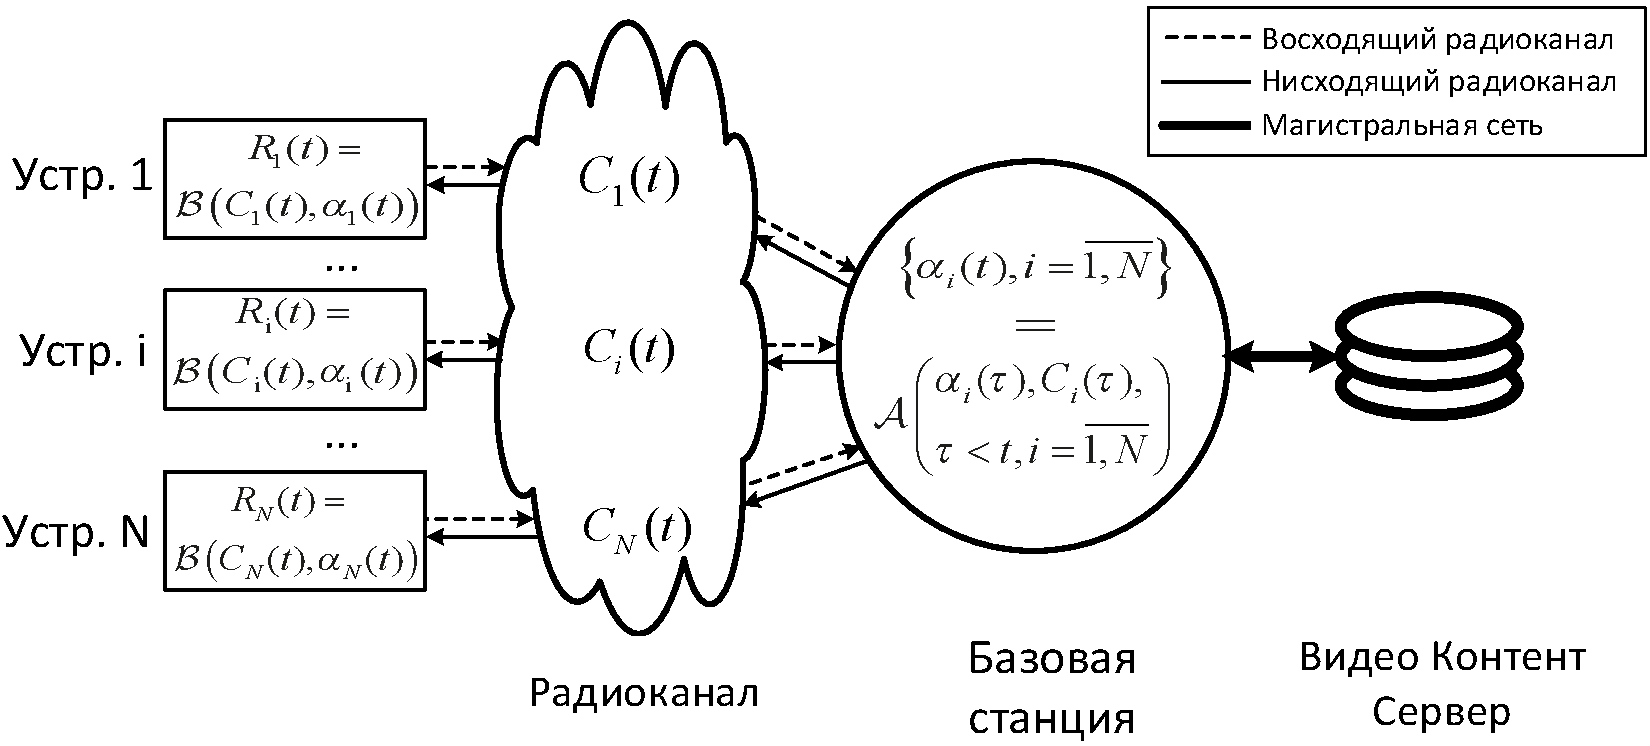
\includegraphics[width=\textwidth]{Chapter2/SystemModelEch.pdf}
\caption{Структура модели передачи видеоданных в централизованных беспроводных сетях}
\label{fig:SystemModel}
\end{center}
\end{figure}

\begin{itemize}
	\item \textit{Формат представления видеоданных}:
		\begin{enumerate}
			\item Все видеопоследовательности разбиты на сегменты одинаковой длительности $d$ секунд;
			\item Каждый сегмент видеоданных $j$ пользователя $i$ представляется в виде последовательности из $P_{i,j}$ пакетов равного объема;
			\item Все видеопоследовательности на видео контент сервер представлены в непрерывном отрезке битовых скоростей (\ref{eq:BitrateConstr});
			\item Длительности видеопоследовательностей $m$, представленных на видео сервере, являются независимыми случайными величинами с конечными математическим ожиданием и дисперсией.
		\end{enumerate}
	\item \textit{Общие характеристики сети передачи информации}:
		\begin{enumerate}
			\item Задержка в восходящем канале считается пренебрежимо малой;
			\item Загрузка сегментов видеоданных начинается незамедлительно в момент отправки запроса.
		\end{enumerate}
	\item \textit{Модель поведения пользователя при просмотре видео}:
		\begin{enumerate}
			\item Паузы между просмотрами $\tau_i$ является независимыми случайными величинами с конечными математическим ожиданием ($\overline{\tau}_i$) и дисперсией.
		\end{enumerate}
	\item \textit{Модель беспроводного канала}:
		\begin{enumerate}
			\item Затухание сигнала при распространении происходит одинаково по всей ширине полосы передачи информации для конкретного пользователя в одном моменте времени;
			\item Кодо-модуляционная схема подбирается таким образом, что вероятность ошибки при передаче информации по беспроводному каналу пренебрежимо мала;
			\item В течении передачи одного пакета $k$ из сегмента $j$ пользователем $i$ в нисходящей линии связи максимально достижимая скорость канала постоянна (\ref{eq:ChannelConst});
			\item Последовательности случайных величин $C^{-1}_{i,1}, C^{-1}_{i,2}, \ldots, i=\overline{1,N}$  формирует эргодические случайные процессы с конечными математическими ожиданиями $E[C_i^{-1}]$ и коэффициентами вариации $\nu^{C}_i$ соответственно.
		\end{enumerate}
	\item \textit{Модель планировщика ресурсов беспроводного канала}:
		\begin{enumerate}
			\item Алгоритм планирования выделяет частотно-временные ресурсы только активным абонентам;
			\item Алгоритм планирования обеспечивает каждому активному абоненту минимальную долю ресурсов беспроводного канала в каждом интервале планирования (\ref{eq:MinGuarPart});
			\item Алгоритм планирования распределяет все доступные частотно-временные ресурсы (\ref{eq:AllResources}).
		\end{enumerate}
	\item \textit{Модель видеоплеера}:
		\begin{enumerate}
			\item Последовательности $R_{i,1}, R_{i,2}, \ldots, i=\overline{1,N}$ формируют эргодические случайные процессы с конечными математическими ожиданиями $E[R_{i}]$ и коэффициентами вариации не превышающими значений $\nu^R_i$ (\ref{eq:SwitchRatio}) соотвественно.
		\end{enumerate}
\end{itemize}
Система допущений завершает представление аналитической модели.

\section{Система передачи видеоданных как система массового обслуживания}
\label{chap2:QueuningNetwork}

Представленная выше аналитическая модель передачи видеоданных описывает достаточно современные тенденции развития телекоммуникационных сетей связи: передача видео и беспроводные сети. Несмотря на данный факт аналогичные системы рассматривались еще в 70-х годах 20-го века, они известны как замкнутые системы массового обслуживания (СМО) с конечным числом абонентов. Далее предлагается краткое описание таких СМО и анализ отличий данных систем от рассматриваемой модели в настоящей работе.

Изначально, СМО с конечным числом абонентов были рассмотрены Шерром в работе \cite{scherr}, в дальнейшем замкнутые СМО с конечным числом абонентов были широко исследованы в работах \cite{adiri, simha, veran}. Общая идеология таких систем состоит в следующем. Абонент отправляет на обслуживающий прибор заявку, которая становится в очередь бесконечного размера. Заявки всех абонентов считаются одинаковыми. Обслуживающий прибор, исходя из зафиксированной дисциплины обслуживания, обрабатывает заявки в очереди. Когда заявка для некоторого абонента была обслужена, то по петле обратной связи для этого абонента будет доставлено уведомление об окончании выполнения заявки. После получения уведомления абонент отправляет следущую заявку в систему через некоторую паузу. В классических СМО с конечным числом абонентов время между получением уведомления об обработки заявки до посылки нового запроса в систему и длительность обслуживания заявки в очереди распределено по экспоненциальному закону.

Важной особенностью подобных систем является то, что в каждый момент времени в очереди на обслуживающем приборе количество заявок не превосходит количество абонентов в сети. Данный факт приводит к тому, что среднее время обслуживания абонентов до точки насыщения системы растет незначительно, а после нее растет линейно, с углом наклона зависящего от интенсивности обслуживания и временем между получением уведомления и отправки новой заявки. Такое поведение среднего времени обслуживания отличается от классических СМО без обратной связи, в которых оно растет экспоненциально после достижения системой точки насыщения, в виду бесконечного роста количества заявок в очереди на обслуживающем приборе.

Опишем систему передачи видеоданных в терминах замкнутых СМО с конечным числом абонентов. Далее будет описана общая логика работы систем передачи видеоданных, в скобках будет представлено название в терминах CМО (рисунок~\ref{fig:QnModel}).

Воспроизводящие устройства (\textit{абоненты}) по восходящему каналу связи отправляют запрос на сегмент видеопоследовательности к контент серверу. Сервер, в свою очередь, отсылает воспроизводящему устройству сегмент видео (\textit{заявку}). Важно отметить, что одновременно одно устройство (\textit{абонент}) может загружать только один сегмент (\textit{заявку}). Все сегменты видеоданных попадают в очереди на базовой станции (\textit{обслуживающем устройстве}). Далее, в соответствии с алгоритмом планирования распределением ресурсов (\textit{дисциплиной обслуживания}), сегменты (\textit{заявки}) из очередей передаются на пользовательское устройства. После получения сегмента воспроизводящее устройство отправит через некоторую паузу новый запрос на контент сервер.

В данной системе запрос на сегмент видеоданных выполняет роль петли обратной связи. В предложенной модели планировщик на базовой станции в каждый момент времени распределяет доли ресурсов канала между активными абонентами. Распределение долей ресурсов канала возможно интерпретировать как разделение времени обслуживания активных абонентов. Следовательно, базовая станция может быть представлена ввиде процессора с разделением времени.

\begin{figure}[htbp]
\begin{center}
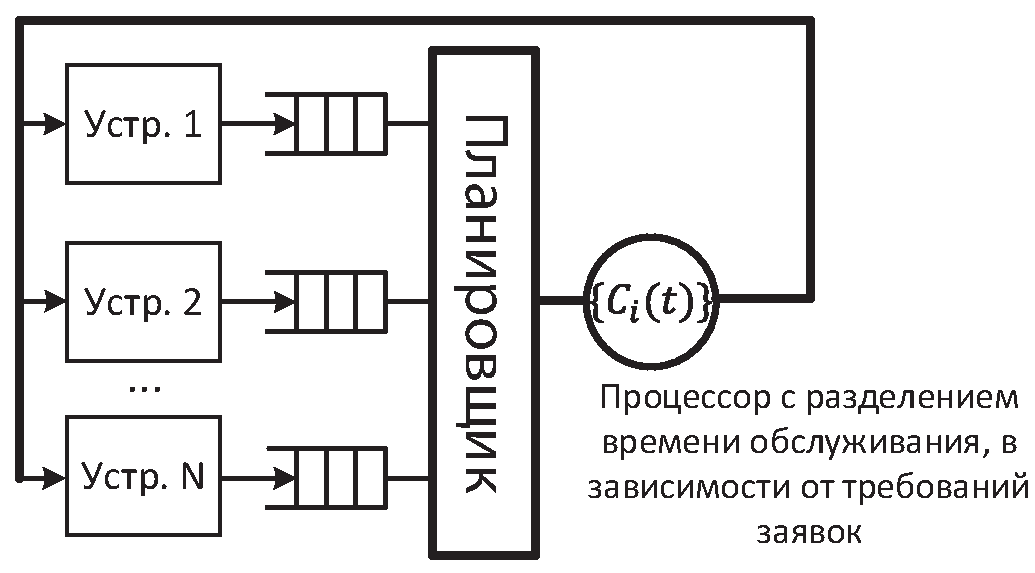
\includegraphics[width=0.7\textwidth]{Chapter2/QnModel.pdf}
\caption{Система передачи видеоданных как замкнутая система массового обслуживания}
\label{fig:QnModel}
\end{center}
\end{figure}

Однако, существует несколько важных отличий систем передачи видеоданных от замкнутых СМО с конечным числом абонентов:
\begin{itemize}
	\item Размер загружаемых сегментов видеоданных изменяется во времени и зависит от скорости загрузки информации, и как следствие, алгоритма планирования;
	\item Длительность интервала времени между получением сегмента и отправки нового запроса не распределено по экспоненциальному закону;
	\item Время передачи сегмента видео через базовую станцию (\textit{время обслуживания заявки}) зависит от его размера и характеристик беспроводного канала всех активных абонентов в текущий момент времени (изменяемая интенсивность обслуживания во времени с дополнительной зависимостью от предыстории).
\end{itemize}

%Данные отличия приводят к невозможности анализа системы передачи видеоданных методами, используемых при анализе классических СМО.

\section{О взаимосвязи параметров системы передачи видеоданных}
\label{chap2:InterrelationVideoParams}

Представленная ранее аналитическая модель описывает важнейшие компоненты и параметры реальной системы передачи видеоданных. Основываясь на данной модели вводится утверждение~\ref{lem:GeneralConstrain}, описывающая основные взаимосвязи между параметрами системы.

\begin{lemma}
\label{lem:GeneralConstrain}
Для всевозможных алгоритмов планирования, удовлетворяющих допущениям, представленных в подразделе \ref{chap2:Scheduler}, следующее неравенство истинно:
\emph{
\begin{equation}
	\label{eq:GeneralConstrain}
	\sum\limits_{i=1}^{N} {\left(1-\nu^R_i\nu^C_i\right)\frac{E[R_i]E[C_i^{-1}]}{q_i + \gamma_i}} \leq 1.
\end{equation}
}
\end{lemma}

\begin{proof}
Рассмотрим процессы в системе передачи видеоданных, когда некоторый пользователь $i$ загружает пакет $k$ из сегмента $j$. В течении загрузки пакета через систему был передан следующий объем информации $\frac{R_{i,j} d }{P_{i,j}}$, который может быть вычислен исходя из наблюдения за скоростью передачи информации в беспроводном канале:
\begin{equation}
	\nonumber
	\int\limits_{t_{i,j,k}}^{t_{i,j,k} + \Delta t_{i,j,k}} S_i(t) dt = C_{i,j,k} \int\limits_{t_{i,j,k}}^{t_{i,j,k} + \Delta t_{i,j,k}}\alpha_i(t) dt = \frac{R_{i,j} d }{P_{i,j}}.
\end{equation}
Перенесем $C_{i,j,k}$ в правую часть последнего равенства и получим долю времени использования канала пользователем $i$ при загрузке $k$-го пакета:
\begin{equation}
	\nonumber
	\int\limits_{t_{i,j,k}}^{t_{i,j,k} + \Delta t_{i,j,k}}\alpha_i(t) dt = \frac{R_{i,j} d }{P_{i,j}}\frac{1}{C_{i,j,k}}.
\end{equation}
Просуммируем левую и правую часть по всем пакетам в сегменте, получим долю времени использования канала пользователем $i$ при загрузке $j$-го сегмента:
\begin{equation}
	\nonumber
	\int\limits_{t_{i,j}}^{t_{i,j} + \Delta t_{i,j}}\alpha_i(t) dt = R_{i,j} d\left( \frac{1}{P_{i,j}}\sum\limits_{k=1}^{P_{i,j}} \frac{1}{C_{i,j,k}}\right),
\end{equation}
где $t_{i,j}$~--~время начала загрузки пользователем $i$ сегмента $j$, $\Delta t_{i,j}$~--~длительность загрузки пользователем $i$ сегмента $j$. Согласно введенным ранее обозначениям (подраздел~\ref{chap2:RadioChannel}) $C_{i,j}^{-1} = P_{i,j}^{-1}\sum\limits_{k=1}^{P_{i,j}} C_{i,j,k}^{-1}$, тогда выражение примет вид:
\begin{equation}
	\nonumber
	\int\limits_{t_{i,j}}^{t_{i,j} + \Delta t_{i,j}}\alpha_i(t) dt = R_{i,j}C_{i,j}^{-1} d.
\end{equation}

%Важно отметить, что в реальной системе величина $P_{i,j}$ принимает значения большие 75-ти. Например, в соответствие с таблицей~\ref{tab:youtubeBr}, для обеспечения разрешения 360p на мобильном устройстве необходима битовая скорость потока $0.45$ Мб/c, минимальная длительность сегмента видеоданных $2$ секунды (таблица~\ref{tab:DashJSParams}), максимальный размер пакета, который может быть передан без фрагментации $1440$ байт. Следовательно, размер одного сегмента $112500$ байт, и он может быть передан за $79$ пакетов. Таким образом, если $C^{-1}_{i,1,1}, C^{-1}_{i,1,2}, \ldots,$ $ C^{-1}_{i,2,1}, C^{-1}_{i,2,2}, \ldots$ формирует эргодический случайный процесс с конечными математическим ожиданием $E[C_i^{-1}]$ и коэффициентом вариации (подраздел~\ref{chap2:Assumptions}), то значение $C_{i,j}^{-1} = E[C_i^{-1}]$.

Тогда доля времени использования канала пользователем $i$ за время $T$:
\begin{equation}
	\label{eq:lemma_1}
	\int\limits_{0}^{T}\alpha_i(t) dt = d\sum\limits_{j=1}^{H_i^T}R_{i,j}C_{i,j}^{-1} + \Delta s_i,
\end{equation}
где $H_i^T$~--~число полностью загруженных сегментов пользователем $i$ в течении времени $T$, $\Delta s_i$~--~длительность видео, загруженного пользователем $i$, но не воспроизведенный плеером. Просуммировав уравнение~(\ref{eq:lemma_1}) для всех пользователей в системе ($i=\overline{1,N}$) и внеся сумму под знак интеграла было получено следующее выражении:
\begin{equation}
	\nonumber
	\int\limits_{0}^{T}\sum\limits_{i=1}^{N}\alpha_i(t)dt = \sum\limits_{i=1}^{N}d\sum\limits_{j=1}^{H_i^T}R_{i,j}C_{i,j}^{-1} + \Delta s,
\end{equation}
где $\Delta s = \sum\limits_{i=1}^{N} \Delta s_i$.

Так как в каждый момент времени $t$ сумма выделенных ресурсов не может превышать единицы, согласно условию (\ref{eq:AllResources}), следовательно $\int\limits_{0}^{T}\sum\limits_{i=1}^{N}\alpha_i(t)dt \leq T$:
\begin{equation}
	\nonumber
	d\sum\limits_{i=1}^{N}\sum\limits_{j=1}^{H_i^T}R_{i,j}C_{i,j}^{-1} + \Delta s \leq T.
\end{equation}
Разделим левую и правую часть неравенства на $T$ и внесем его под первый знак суммы, так как $T>0$ знак неравенства не изменится.
\begin{equation}
	\nonumber
	\sum\limits_{i=1}^{N}{\frac{d\sum\limits_{j=1}^{H_i^T}R_{i,j}C_{i,j}^{-1} + \Delta s_i}{T}} \leq 1.
\end{equation}
Для каждого пользователя время пребывание в системе состоит из буферизаций, просмотров и пауз между просмотрами видео: $T = b_i^T + w_i^T + p_i^T $, следовательно последнее неравенство представляется в следующем виде:
\begin{equation}
	\nonumber
	 \sum\limits_{i=1}^{N}{\frac{d\sum\limits_{j=1}^{H_i^T}R_{i,j}C_{i,j}^{-1} + \Delta s_i}{b_i^T + w_i^T + p_i^T}} \leq 1.
\end{equation}
Так как длительность просмотра равняется длительности всех загруженных сегментов, $w_i^T = H_i^T d,i=\overline{1,N}$:
\begin{equation}
	\nonumber
	\sum\limits_{i=1}^{N}\frac{w_i^T \frac{1}{H_i^T}\sum\limits_{j=1}^{H_i^T}R_{i,j}C_{i,j}^{-1} + \Delta s_i}{b_i^T + w_i^T + p_i^T} \leq 1.
\end{equation}
Разделив числитель и знаменатель левой части полученного выражения на $w_i^T$ и устремим время в бесконечность ($T\rightarrow\infty$). Для каждого абонента $i = \overline{1,N}$ воспользуемся определением $q_i$ и получим следующее выражение:
\begin{equation}
	\nonumber
	\sum\limits_{i=1}^{N}\frac{E\left[R_{i}C_{i}^{-1}\right] }{q_i + \gamma_i} \leq 1.
\end{equation}
Данный переход возможен так как последовательности $R_{i,1}, R_{i,2}, \ldots$ и $C_{i,1}, C_{i,2}, \ldots i=\overline{1,N}$ формируют эргодические случайные процессы с кончеными первыми двумя моментами (подраздел~\ref{chap2:Assumptions}).

Рассмотрим более подробно значение, получившее в числителе: $E\left[R_{i}C_{i}^{-1}\right]$. Важно отметить, что битовая скорость потока $R_i$ для каждого пользователя выбирается в зависимости от оценки качества канала, которая определяется максимально достижимой скоростью канала $C_i$. Следовательно, значения $R_i$ и $C_i$ являются зависимыми величинами, и математическое ожидание их произведения:
\begin{equation}
	\nonumber
	E\left[R_{i}C_{i}^{-1}\right] = E\left[R_{i}\right]E\left[C_{i}^{-1}\right] + r \left(R_i, C_{i}^{-1}\right) \sigma[R_i]\sigma[C_i^{-1}],
\end{equation}
где $r \left(R_i, C_{i}^{-1}\right)$ является коэффициентом корреляции между величинами $R_i$ и $C_{i}^{-1}$. По определению значение $r \left(R_i, C_{i}^{-1}\right)$ принимает значения в отрезке $[-1, 1]$, следовательно:
\begin{equation}
	\nonumber
	 E\left[R_{i}\right]E\left[C_{i}^{-1}\right] - \sigma[R_i]\sigma[C_i^{-1}] \leq E\left[R_{i}C_{i}^{-1}\right].
\end{equation}
Исходя из данного факта:
\begin{equation}
	\nonumber
	\sum\limits_{i=1}^{N} {\left(1-\nu^R_i\nu^C_i\right)\frac{E[R_i]E[C_i^{-1}]}{q_i + \gamma_i}} \leq 1.
\end{equation}
Таким образом, утверждение \ref{lem:GeneralConstrain} доказано.
\end{proof}

Результат, представленный в утверждении \ref{lem:GeneralConstrain}, описывает взаимосвязь между всеми характеристиками сети передачи видеоданных от особенностей модели поведения пользователя ($\gamma_i$, $q_i$) и характеристик видеопотока ($E[R_i]$), до аспектов работы радиоканала ($E[C_i^{-1}]$) для всех пользователей в сети. Полученное выражение возможно использовать в качестве ограничения на достижимый объем ресурсов радиоканала при оптимизации передачи видеоданных в беспроводных централизованных сетях.

В дальнейшем, для упрощения математических выкладок в качестве обозначений $E[R_i]$ и $E[C^{-1}_i]$ будут использоваться конструкции $\tilde{R}_i$ и $\tilde{C}^{-1}_i$ соответственно.

\section{Выводы по разделу}

В данном разделе была предложена модель передачи видеоданных в современных централизованных беспроводных сетях. Предложенная модель описывает все важнейшие компоненты существующих сетей: магистральная и опорная сети передачи информации, базовая станция (структура беспроводного канала и алгоритм распределения его ресурсов) модель видеотрафика (формат представления видео и аспекты работы воспроизводящего устройства). Так же модель системы передачи видеоданных в беспроводных централизованных сетях была рассмотрена как замкнутая система массового обслуживания с конечным числом абонентов. В завершении раздела был представлен результат, описывающий основополагающие взаимосвязи между всеми характеристиками сети передачи видеоданных.

Основные результаты раздела возможно сформулировать следующим образом:
\begin{itemize}
	\item Предложена модель передачи видеоданных в беспроводных централизованных сетях, включающая в себя:
	\begin{itemize}
		\item Модель опорной и магистральной сети передачи информации (подраздел~\ref{chap2:GeneralOverview});
		\item Модель беспроводного канала связи (подраздел~\ref{chap2:RadioChannel});
		\item Модель работы базовой станции и планировщика ресурсов беспроводного канала (подраздел~\ref{chap2:Scheduler});
		\item Модель воспроизводящего устройства и видеотрафика (подраздел~\ref{chap2:VideoTrafficModel});
		\item Систему допущений (подраздел~\ref{chap2:Assumptions}).
	\end{itemize}
	\item Проведен анализ беспроводных систем перечи видео как замкнутых систем массового обслуживания с конечным числом абонентов (подраздел~\ref{chap2:QueuningNetwork});
	\item Представлена взаимосвязь между всеми всеми характеристиками сети передачи видеоданных (подраздел~\ref{chap2:InterrelationVideoParams}).
\end{itemize}